\documentclass[fleqn]{article}

\usepackage{polski}
\usepackage[utf8]{inputenc}
\usepackage[polish]{babel}
\usepackage{parskip}
\usepackage{icomma}
\usepackage[a4paper,includeheadfoot,margin=1.27cm]{geometry}
\usepackage{float}
\usepackage{graphicx}
\usepackage{amsmath}
\usepackage[hypcap=true]{subcaption}
\usepackage{xcolor}
\usepackage{transparent}
\usepackage{listings}
\usepackage[colorlinks=true, linkcolor=blue, pdfborder={0 0 0}]{hyperref}

\renewcommand\thesection{\arabic{section}.}
\renewcommand\thesubsection{\alph{subsection})}
\renewcommand\thesubsubsection{}
\newcommand\square[1]{
	\fcolorbox{black}{#1}{\rule{0pt}{6pt}\rule{6pt}{0pt}}
}

\brokenpenalty=1000
\clubpenalty=1000
\widowpenalty=1000

\title{\textbf{STP} \\ \large Projekt II - Zadanie 2.39}
\author{Marcin Skrzypkowski \\ nr albumu 283419}

\begin{document}

\maketitle

\setcounter{page}{0}
\thispagestyle{empty}

\pagebreak
\setcounter{page}{1}


\tableofcontents
\pagebreak


\begin{center}

	Obiekt regulacji jest opisany poniższą transmitancją

	\Large{\textbf{G($s$)=}$\frac{K_oe^{-T_os}}{(T_1s+1)(T_2s+1)}$}
\end{center}

\begin{table}[H]
	\centering
	\label{my-label}
	\begin{tabular}{|l|l|l|l|l|}\hline
		% &K & T_1 & T_2 &   \alpha_1 & \alpha_2 & \alpha_3 & \alpha_4 \\ \hline
		% &$5.5$ & $7$ & $7$ &$-0.12$ & $0.4$ & $0.25$ & $0.2$\\ \hline
		$K_o$ & $T_o$ &$T_1$ &  $T_2$   \\ \hline
		$4.5$ & $5$ & $1.87$ &$5.31$\\ \hline
	\end{tabular}
	\caption{Wartości parametrów obiektu regulacji}
\end{table}

\section{Wyznaczenie transmitancji dyskretnej}

W celu wyznaczenia transmitancji dyskretnej obiektu wykorzystana została funkccja \textit{c2d}. Po ustaleniu okresu próbkowania na $0.5$s i wykorzystaniu ekstrapolatora zerowego rzędu porównano odpowiedzi skokowe obiektu ciągłego i dyskretnego. Ekstrapolator spełnia równanie:
{\Large
\begin{equation}
	G(z)=\frac{1-z^{-1}}{z}\mathcal{Z}\bigg\{\frac{G(s)}{s}\bigg\}
\end{equation}

}

Transmitancja dyskretna ma postać
{\Large
\begin{equation}
	G(z)=z^{-10}\frac{0.05029z+0.04458}{z^2-1.676z+0.6966}
\end{equation}
}

Poniższe wyniki potwierdzają prawidłowe wyznaczenie obiektu dyskretnego, gdyż obie odpowiedzi się pokrywają.

\begin{figure}[H]
	\centering
	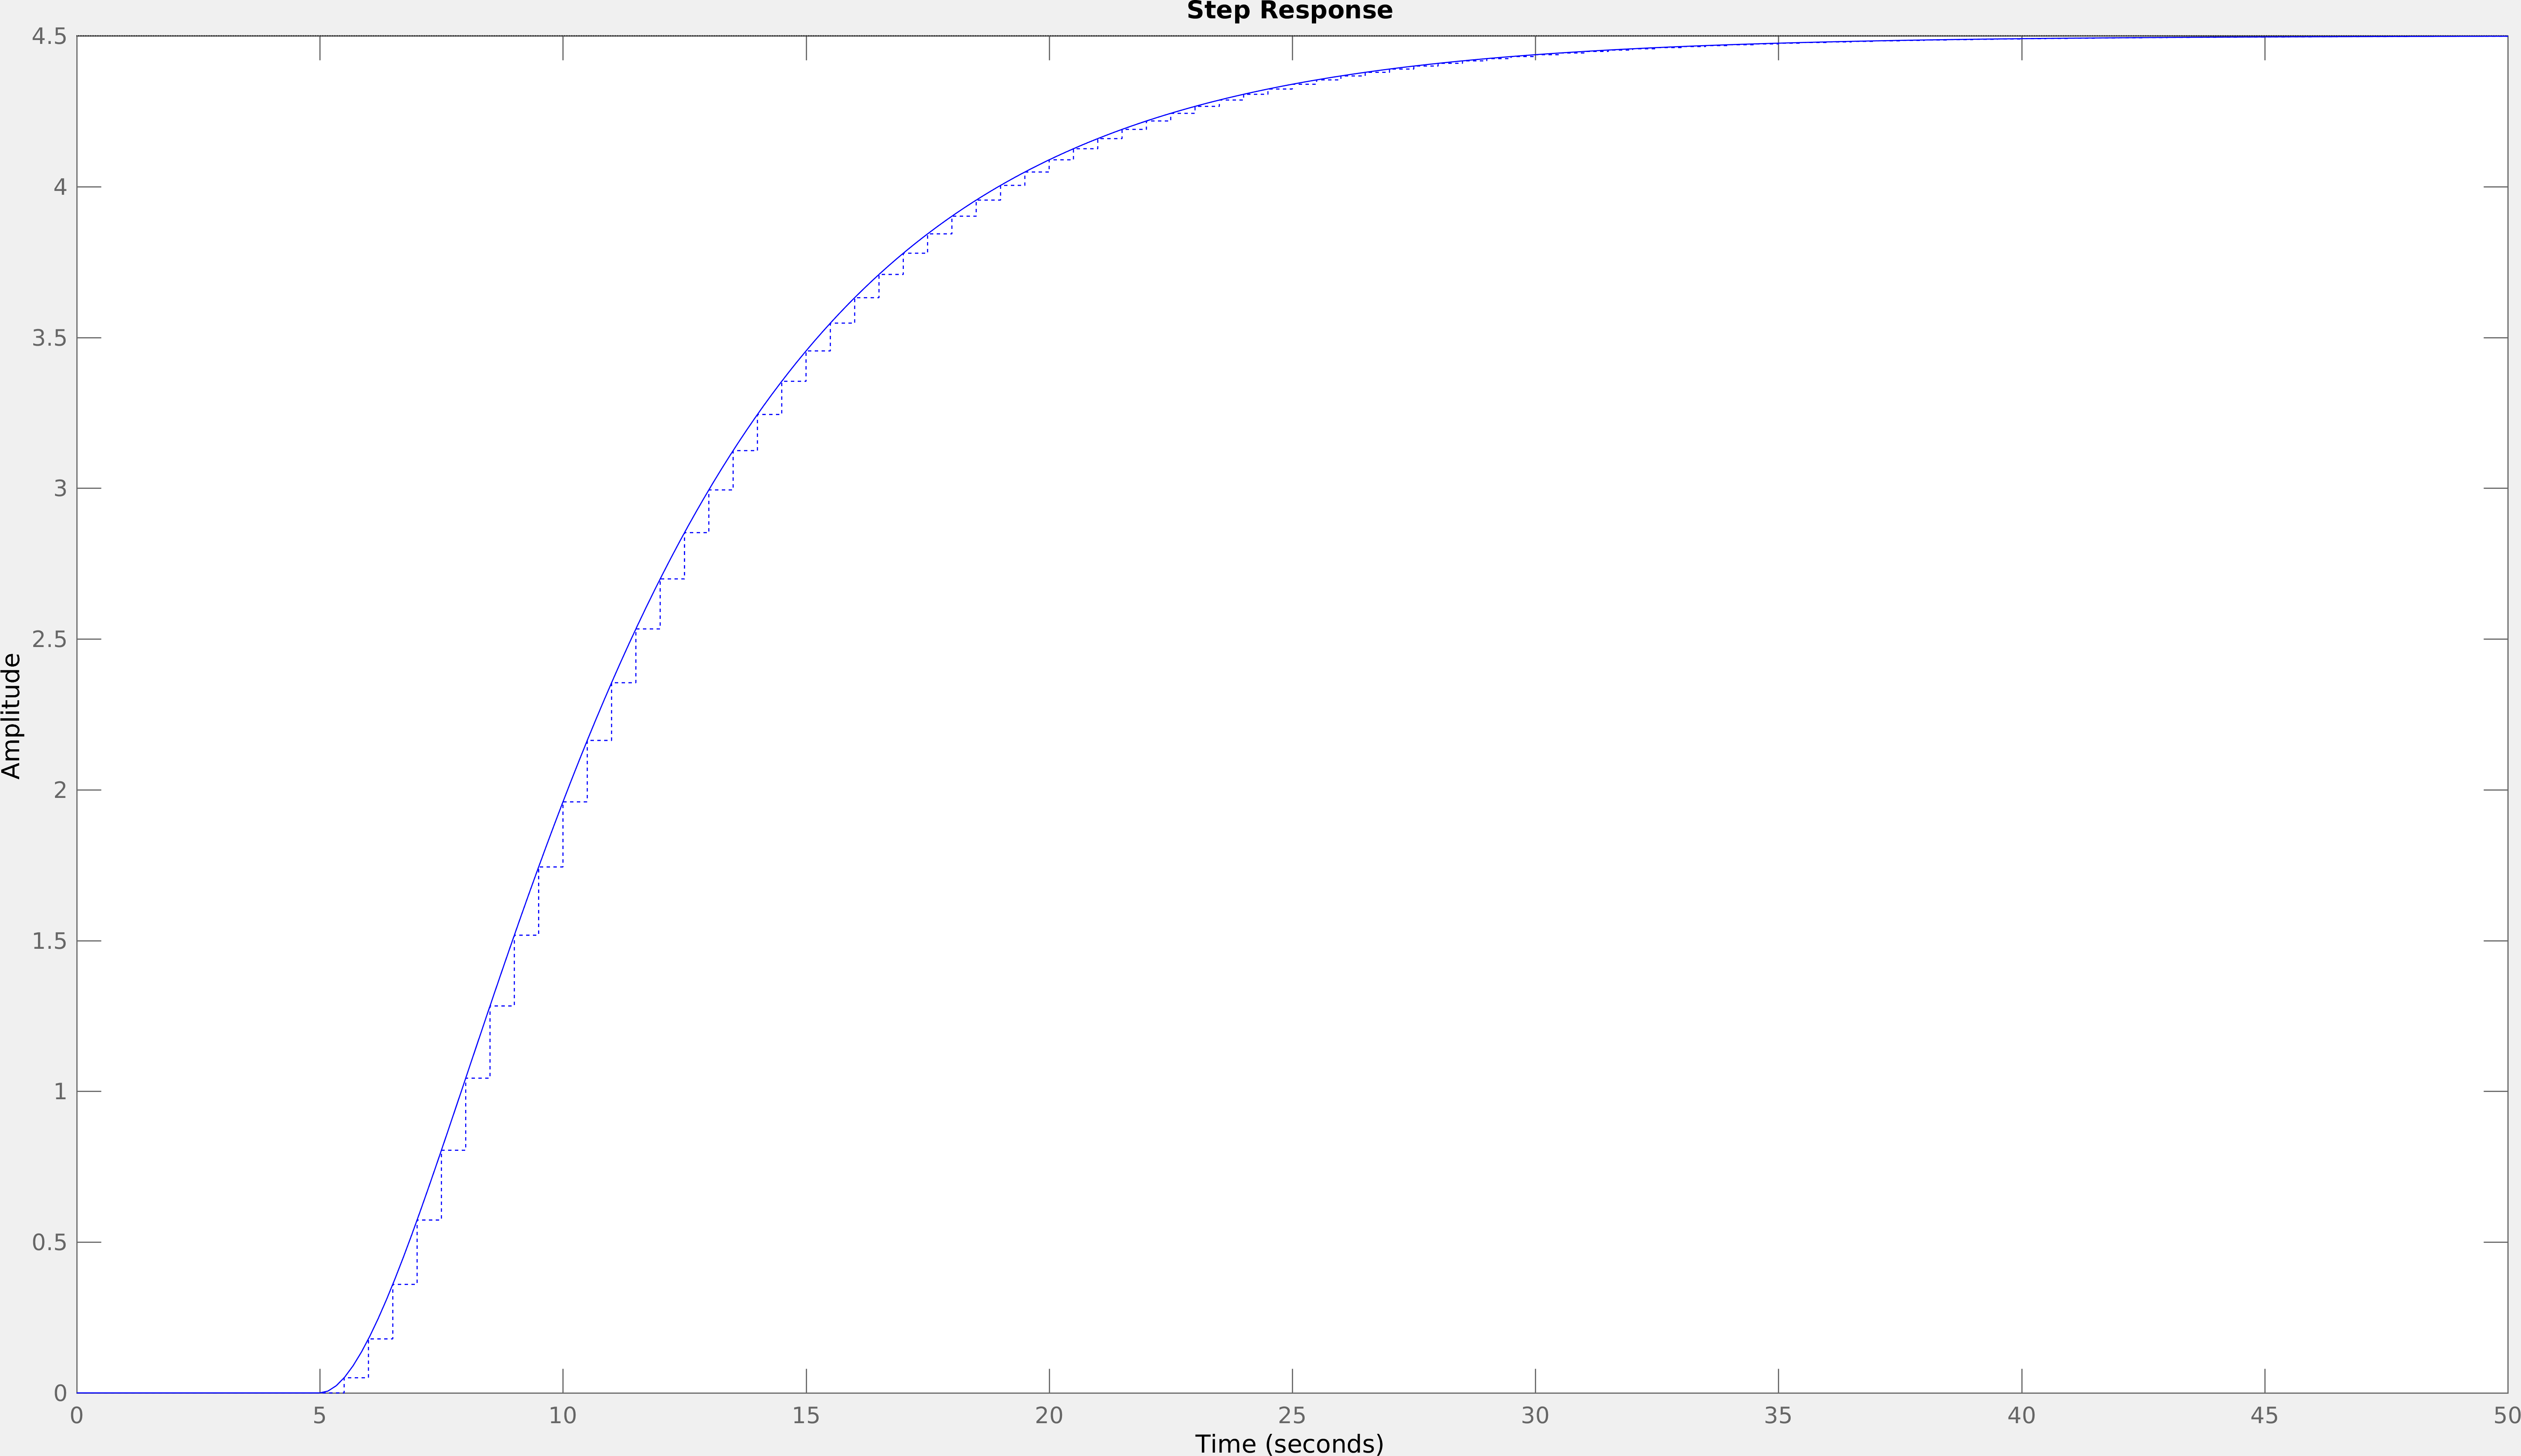
\includegraphics[width=\textwidth]{scripts/odpowiedzskok.png}
	\caption{odpowiedź skokowa obiektu ciągłego i dyskretnego}
	\label{}
\end{figure}

 Ekstrapolator zerowego rzędu nie jest przybliżeniem obiektu regulacji jak to ma miejsce w przypadku emulacji przykładowo wzorem Eulera, lecz pozwala dobierać regulator cyfrowy bezpośrednio na niezaokrąglonej odpowiedzi obiektu.

 Następnie wyznaczono wartości wzmocnienia statycznego trnamsitancji ciągłej i dyskretnej korzystając z następujących wzorów:
{\Large
\begin{equation}
	K_s=\lim_{s\to 0}sX(s)= 4.5
\end{equation}
\begin{equation}
	K_z=\lim_{z\to 1}(1-z^{-1})Y(z)\approx 4.6053
\end{equation}
}

odpowiedzi skokowe obu transmitancji mają praktycznie takie same wartości z dokłądnością do współczynników wyznaczonych przez funkcję \textit{c2d}.

\section{Równanie różnicowe}

Równanie różnicowe postaci
{\Large
\begin{equation}
		y(k)=\sum\limits_{i=1}^{n}b_iy(k-i)+\sum\limits_{i=1}^mc_iu(k-i)
\end{equation}
}

Wyznacza się przez przekształcenie postaci transmitancji dyskretnej, która jest równa stosunkowi wyjścia obiektu do jego sterowania

{\Large
\begin{equation}
	\frac{Y(z)}{X(z)}=\frac{c_mz^m + c_{m-1}z^{m-1}+\dots+c_1z+c_0}{z^n+b_{n-1}z^{n-1}+\dots+b_1z+b_0}
\end{equation}}

Po przekształceniu równanie ma postać

{\Large
\begin{equation}
	y(k)=0.05029u(k-11)+0.04458u(k-12)+1.676y(k-1)-0.6966y(k-2)
\end{equation}
}
\pagebreak

\section{Ciągły regulator PID}

Ciągły równoległy regulator PID opisany jest rónwaniem transmitacji

{\Large
\begin{equation}
	U(s)=K_r(1+\frac{1}{T_is}+T_ds)E(s)
\end{equation}
}

W celu dobrania nastaw wykorzystano metodę Zieglera-Nicholsa. Algorytm wygląda następująco:
\begin{itemize}
	\item wyłączyć człony całkujący i różniczkujący regulatora
	\item dobrać możliwe dużą wartość współczynnika członu proporcjonalnego ($K_k$), aby dotrzeć do granicy stabilności obiektu przy odpowiedzi skokowej
	\item zbadać okres oscylacji wyznaczonych w poprzednim punkcie ($T_k$)
	\item obliczyć nastawy regulatora $K_r=0.6K_k, T_i=0.5T_k, T_d=0.12T_k$
\end{itemize}

Mimo wielu prób nie udało się osiągnąć bardziej satysfakcjonującego wyniku regulacji niż przy nastawach wyznaczonych metodą Zieglera-Nicholsa. Poniżej znajduje się wykres kilku iteracji regulacji dla różnych wartości $T_i$ oraz $T_d$

\begin{figure}[H]
	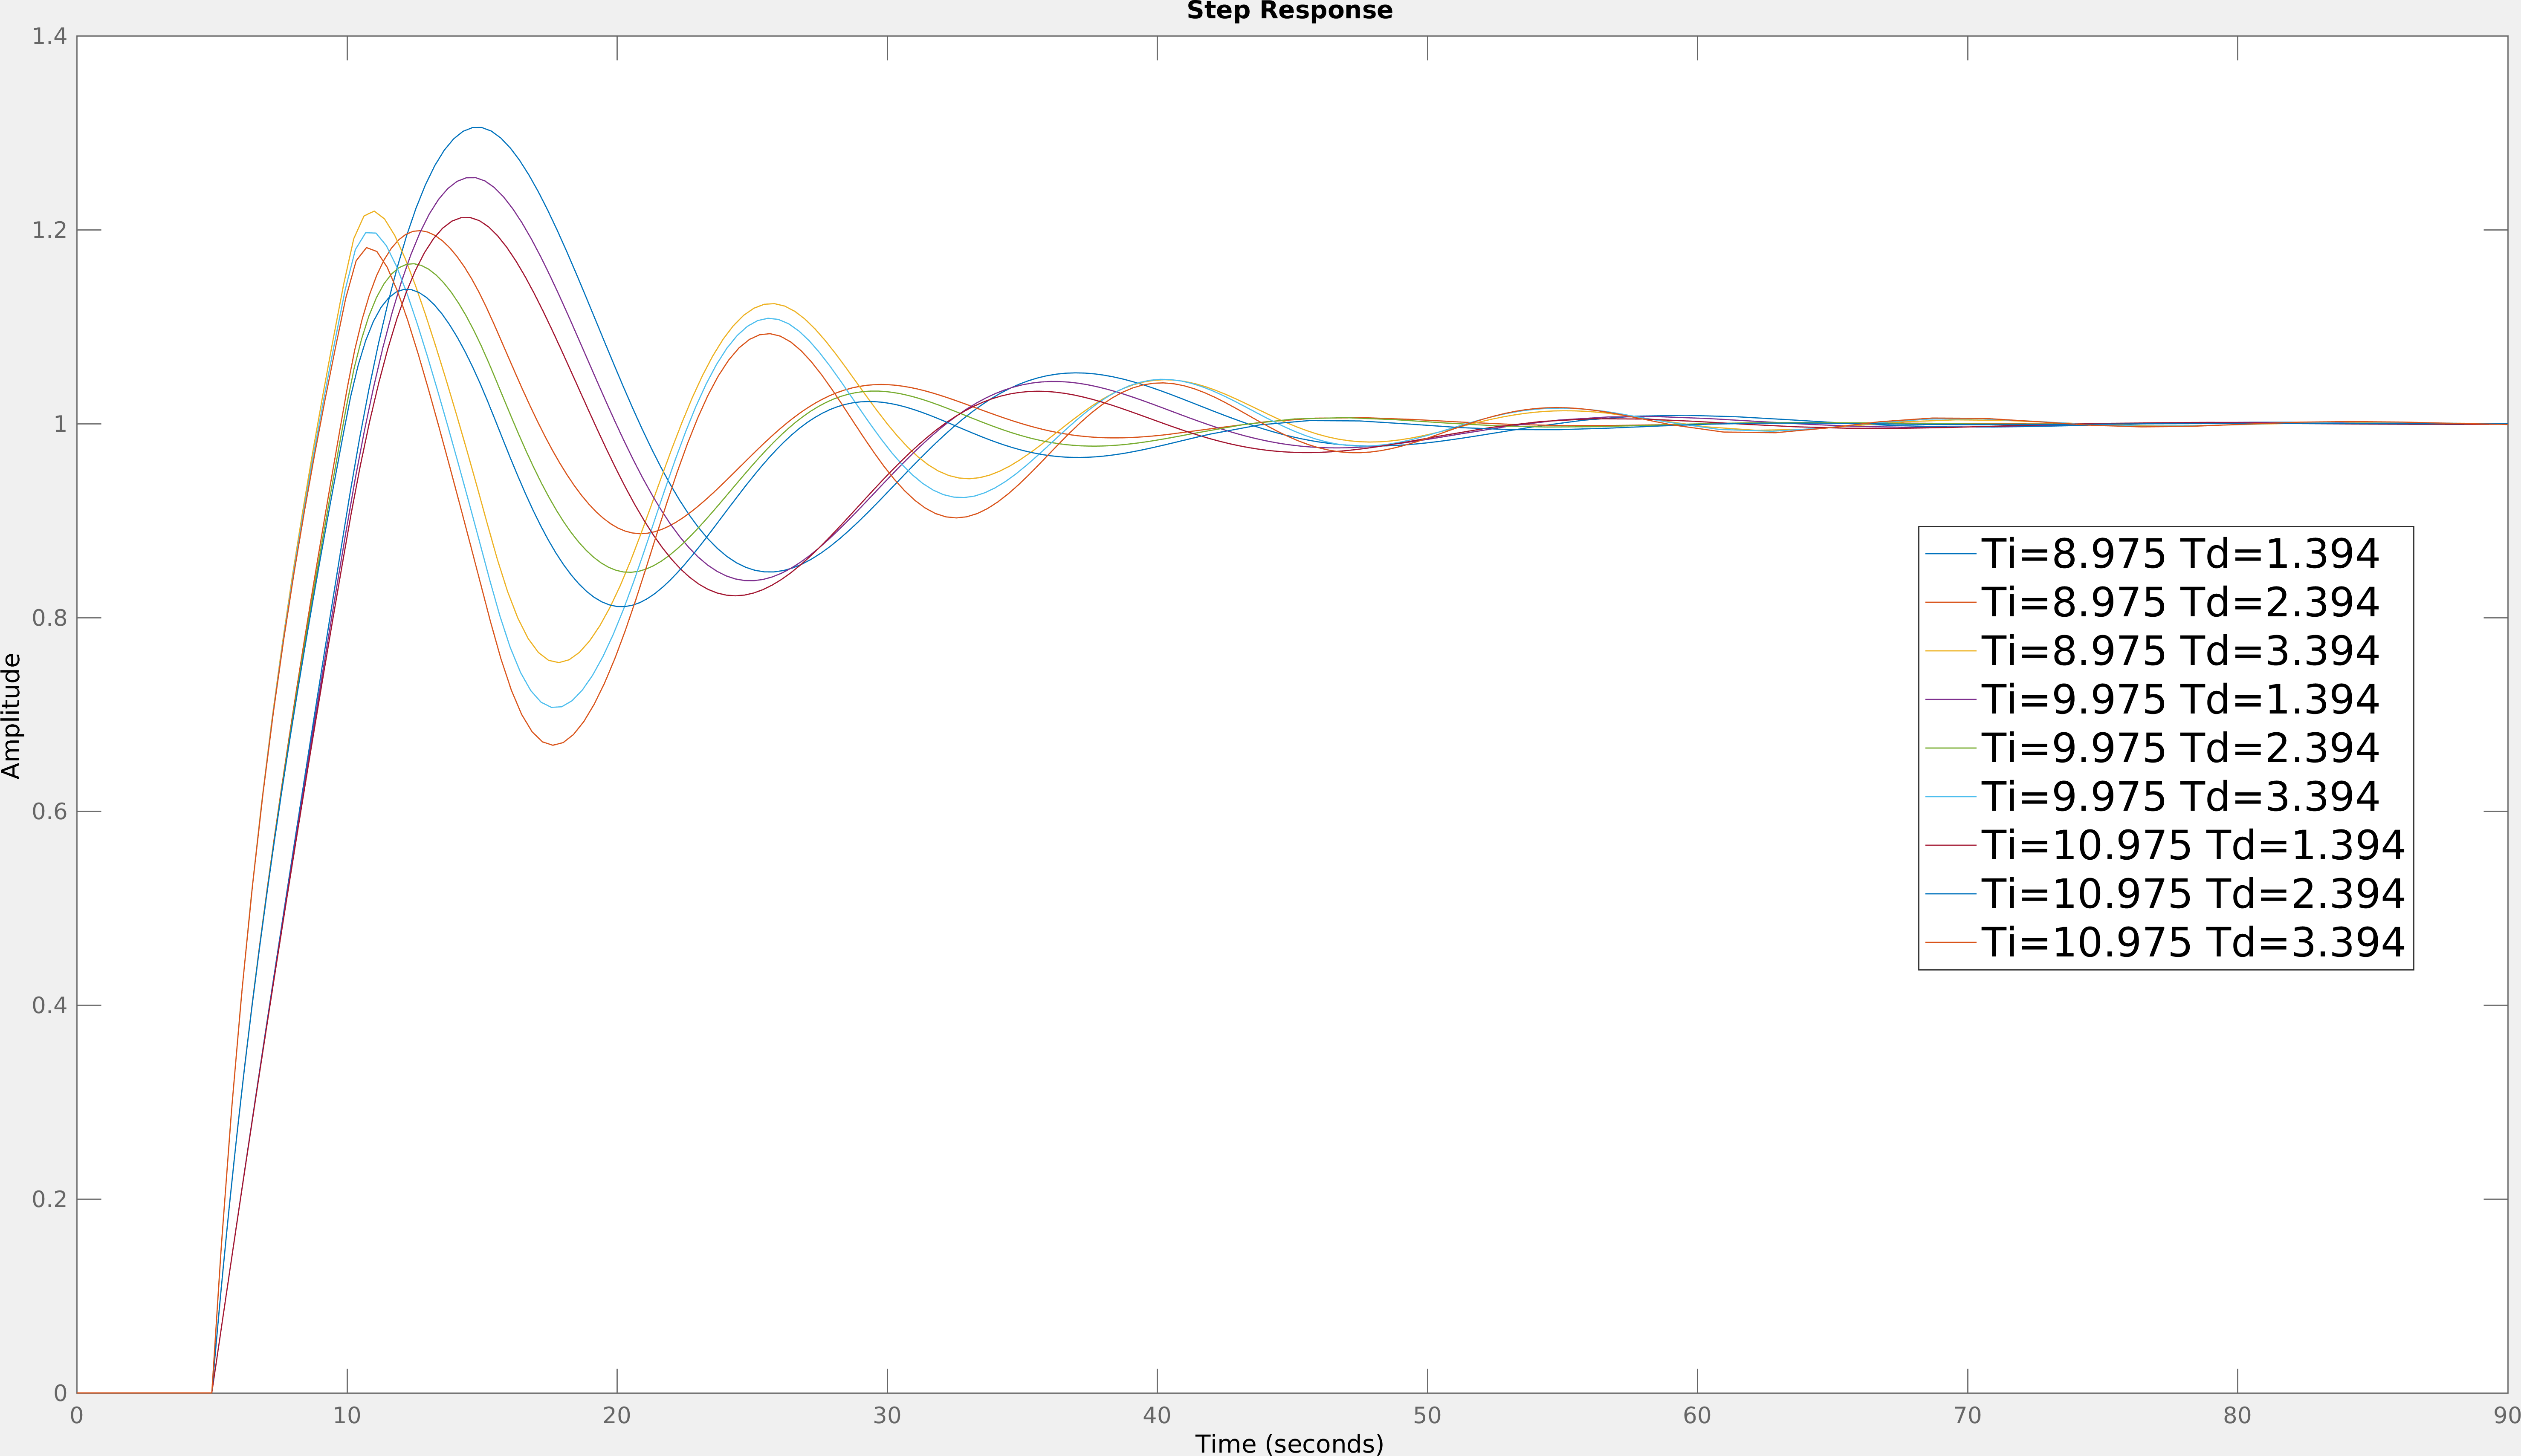
\includegraphics[width=\textwidth]{scripts/odpowiedzskokZN.png}
	\caption{Próba dostrojenia regulatora PID, $K_k = 0.5012$}
\end{figure}

Obliczone wartości współczynników po algorytmie Zieglera-Nicholsa:
\begin{itemize}
	\item $K_r = 0.5019$
	\item $T_i = 9.975$
	\item $T_d = 2.394$
\end{itemize}
\pagebreak
Po eksperymentowaniu również z wartością współczynnika proporcjonalnego udało się otrzymać następujące wyniki

\begin{figure}[H]
	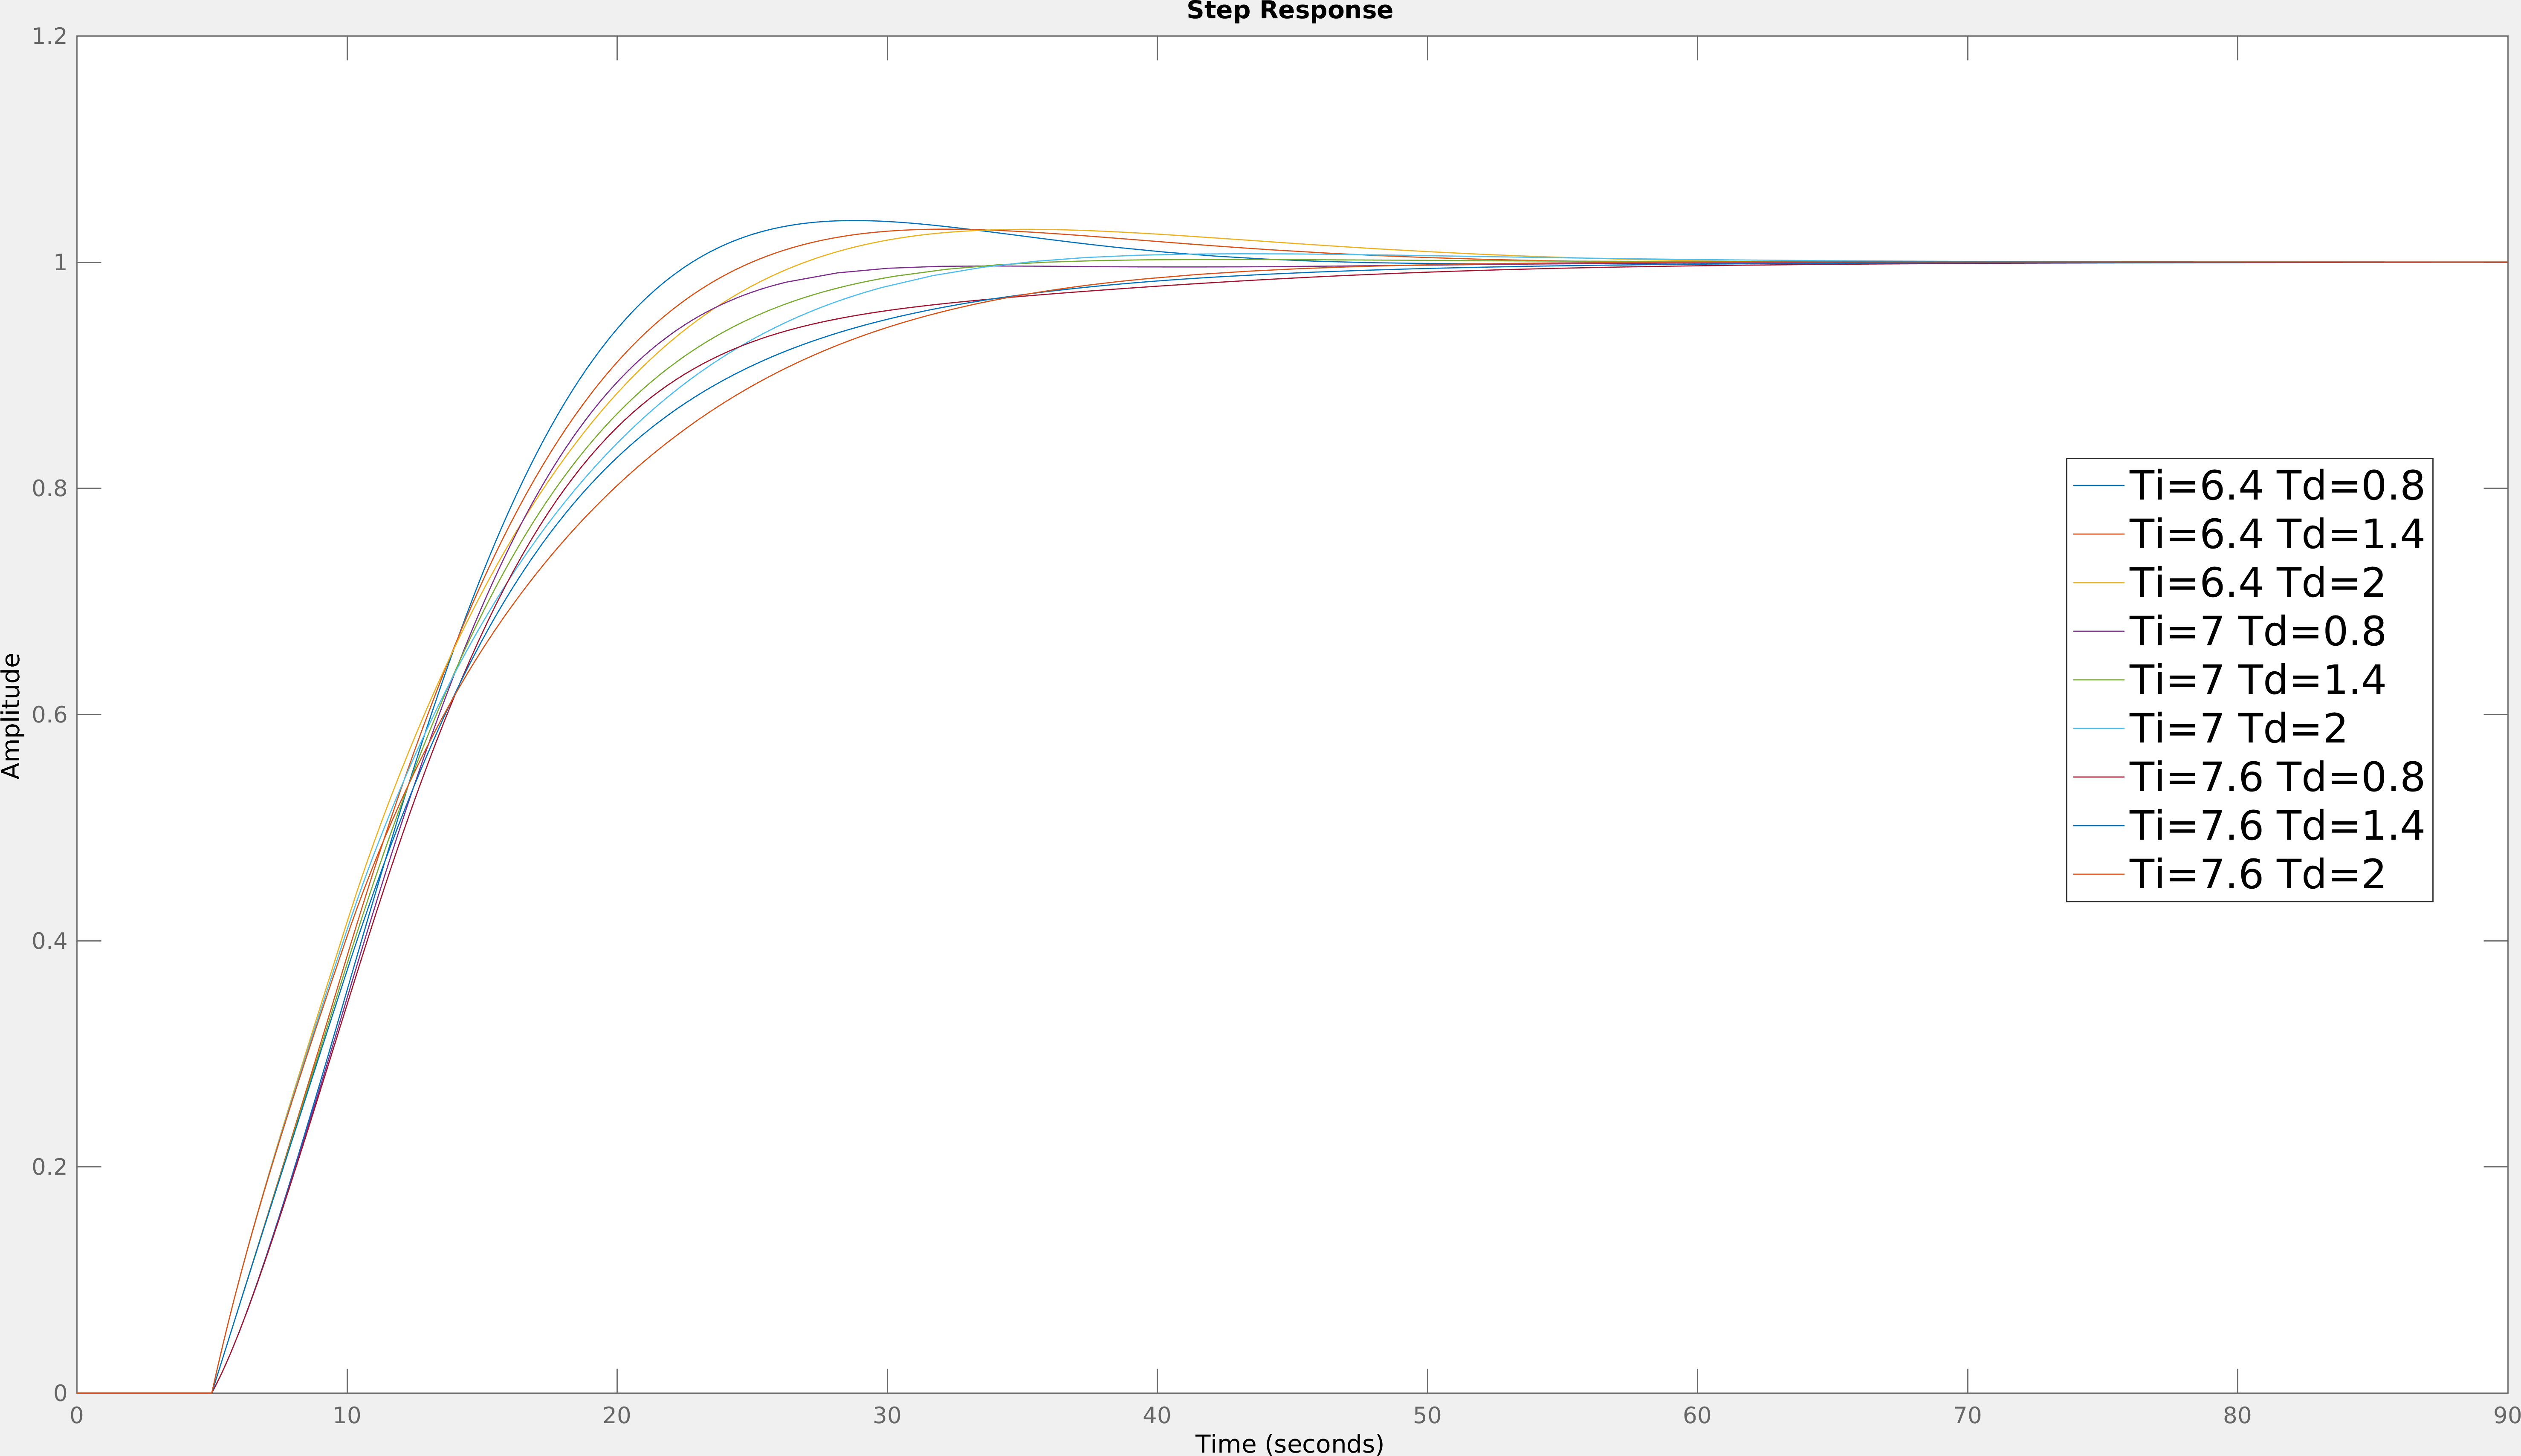
\includegraphics[width=\textwidth]{scripts/odpowiedzskokM.png}
	\caption{Odpowiedź skokowa po zmniejszeniu współczynnika $K_r$ do 0.2}
\end{figure}

Najlepsze nastawy, jakie udało się uzyskać, mają wartości
\begin{itemize}
	\item $K_r = 0.2$
	\item $T_i = 7$
	\item $T_d = 0.8$
\end{itemize}

Przemawiają za nimi brak oscylacji oraz zdecydowanie krótszy czas regulacji.

Następne doświadczenia będą przeprowadzane w dwóch przypadkach, dla nastaw wyznaczonych metodą Z-N oraz najlepszych znalezionych.

Następnym zadaniem było wyznaczenie nastaw regulatora cyfrowego. Ma on postać
{\Large
\begin{equation}
	U(k)=r_2E(k-2)+r_1E(k-1)+r_0E(k)
\end{equation}
}

gdzie
{\Large
\begin{equation}
	r_0=K_r(1+\frac{T_p}{2T_i}+\frac{T_d}{T_p})\\
	r_1=K_r(\frac{T_p}{2T_i}-2*\frac{2T_d}{T_p}-1)\\
	r_2=K_r\frac{T_d}{T_p}
\end{equation}
}
$T_p$ to okres próbkowania, w tym przypadku wynosi on $0.5$s.
\pagebreak
\subsection{Nastawy Zieglera-Nicholsa}

Po podstawieniu wyznaczonych wcześniej wartości wspołczynników otrzymano następujące wartości parametrów regulatora cyfrowego
\begin{itemize}
	\item $r_0 = 1.7481$
	\item $r_1 = -3.1729$
	\item $r_2 = 1.4398$
\end{itemize}


\subsection{Nastawy poprawione}
Poniżej znajdują się wartości współczynników obliczonych na podstawie poprawionego regulatora ciągłego.
\begin{itemize}
	\item $r_0 = 0.5271$
	\item $r_1 = -0.8329$
	\item $r_2 = 0.32$
\end{itemize}

\subsection{Porównanie}
\begin{figure}[H]
	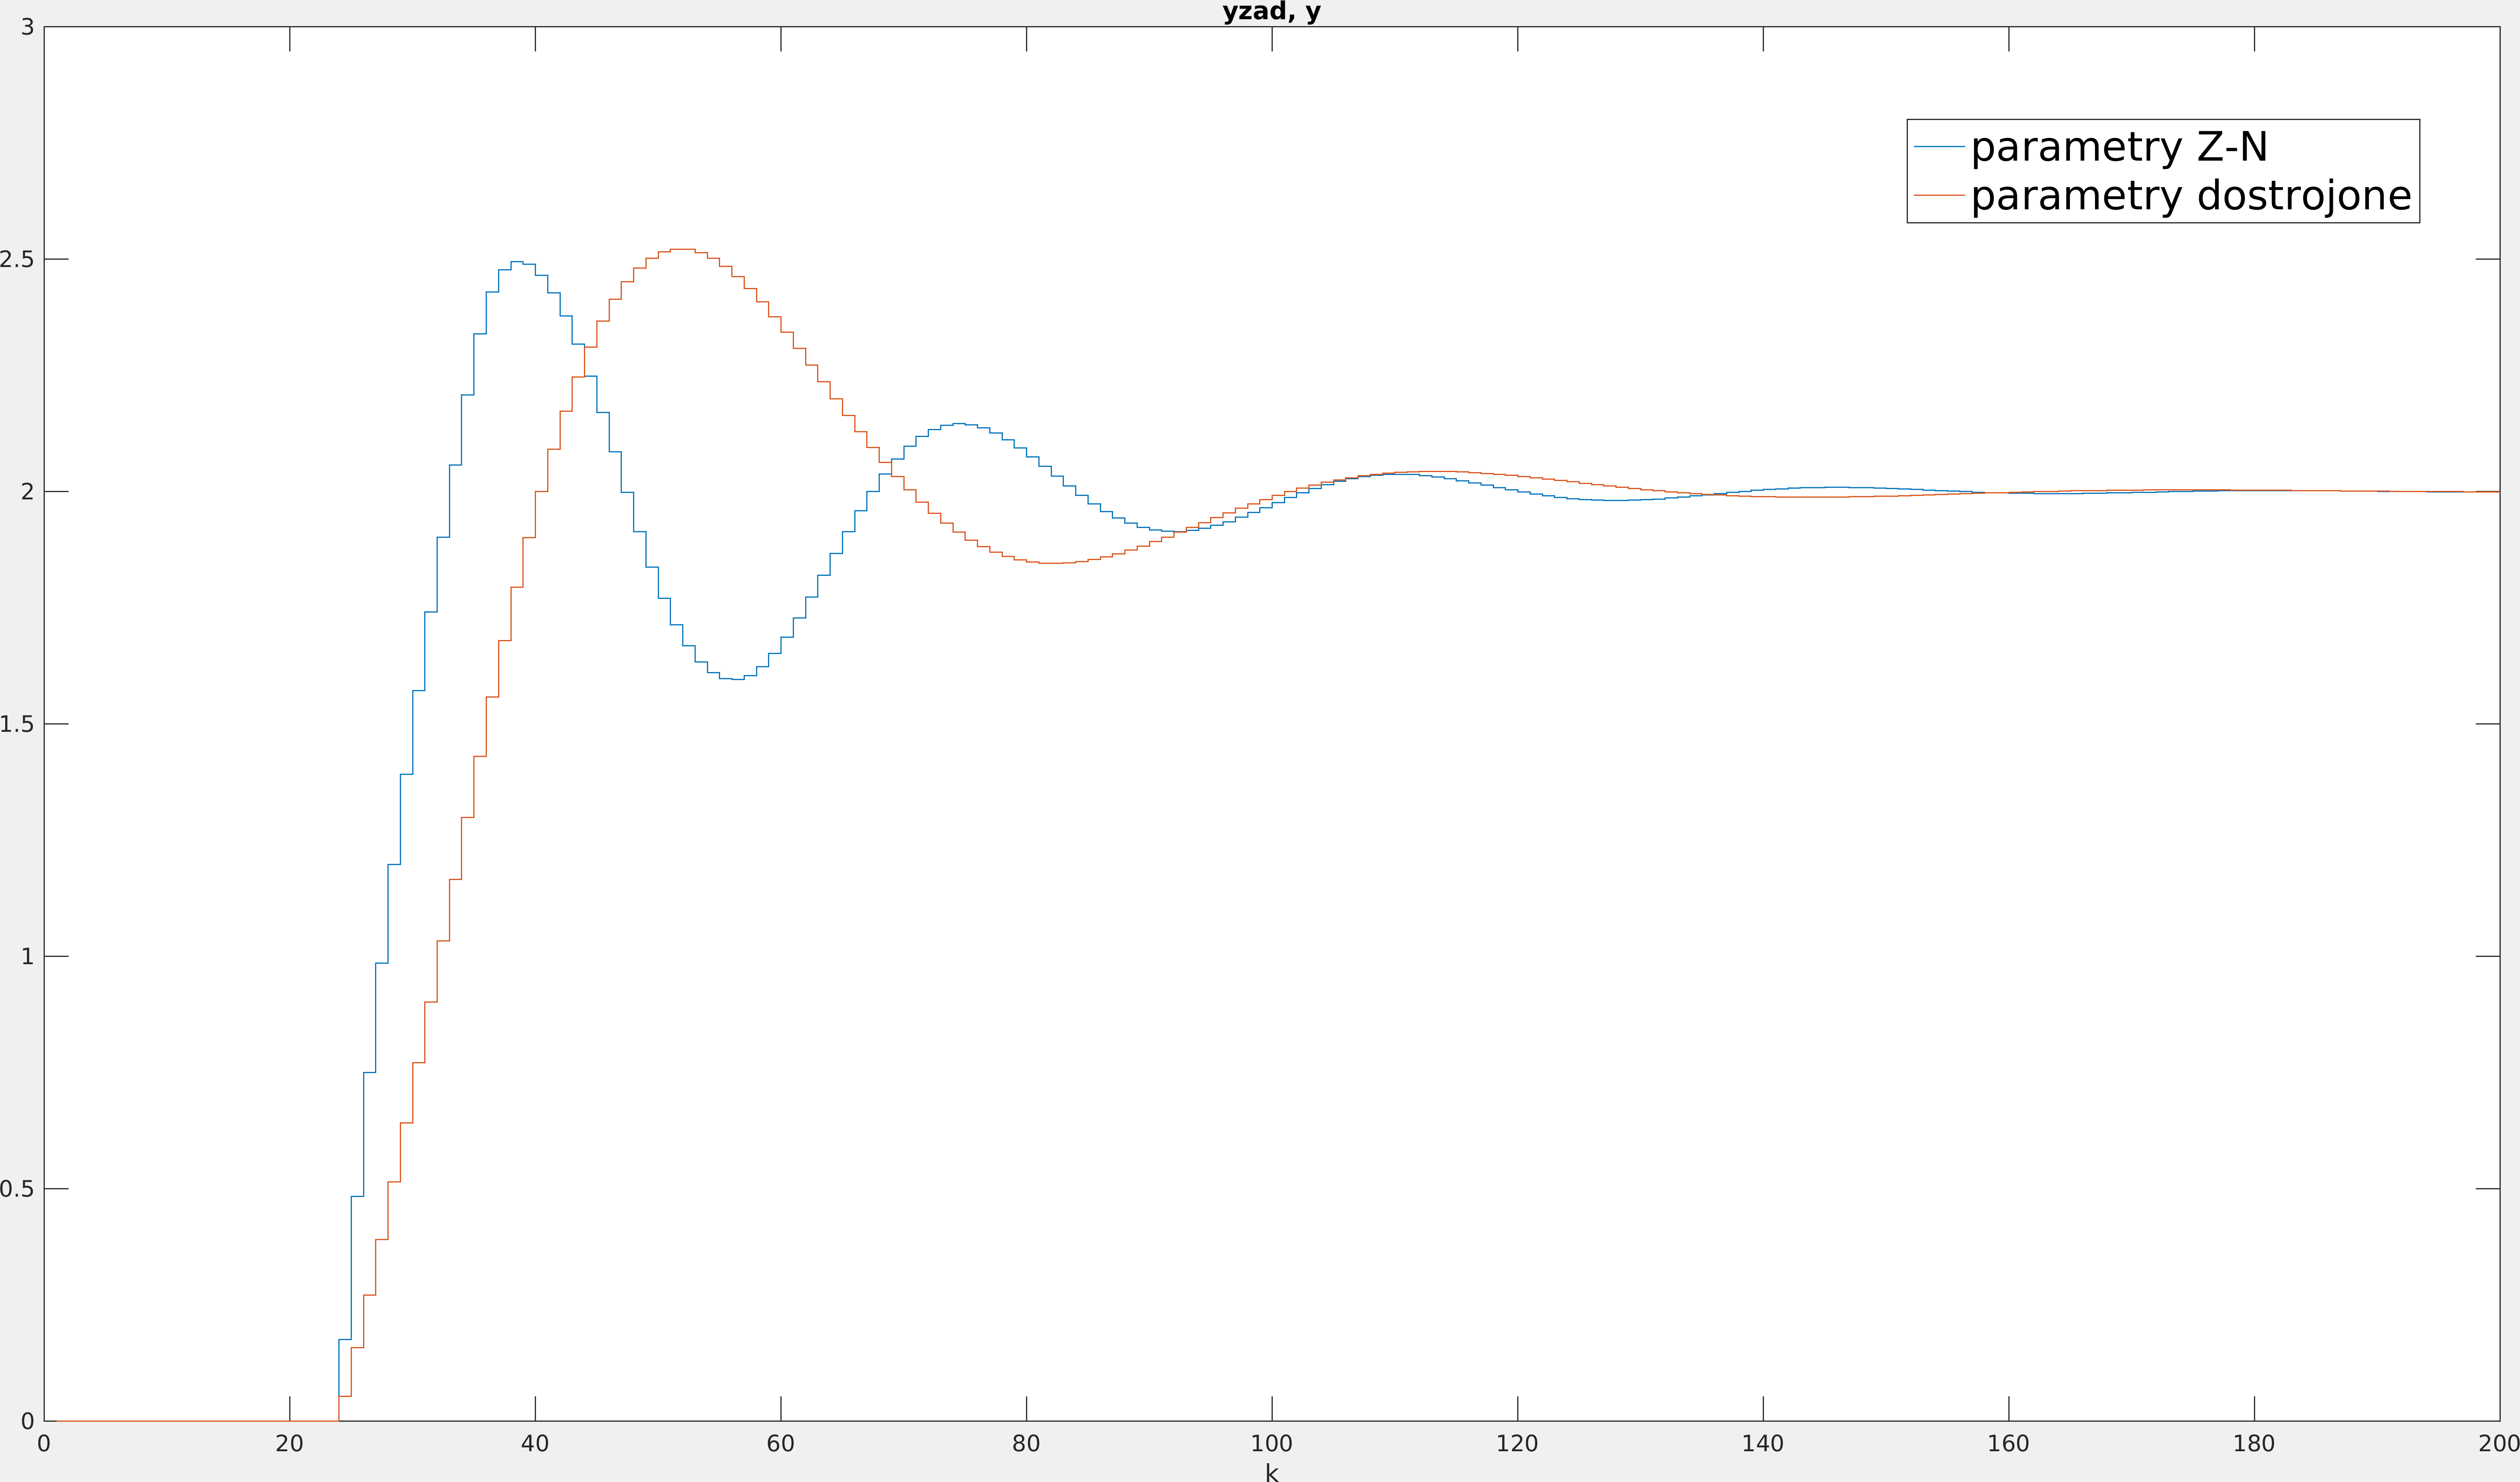
\includegraphics[width=\textwidth]{scripts/dyskretwyj.png}
	\caption{wyjście obiektu regulacji cyfrowej}
\end{figure}

\begin{figure}[H]
	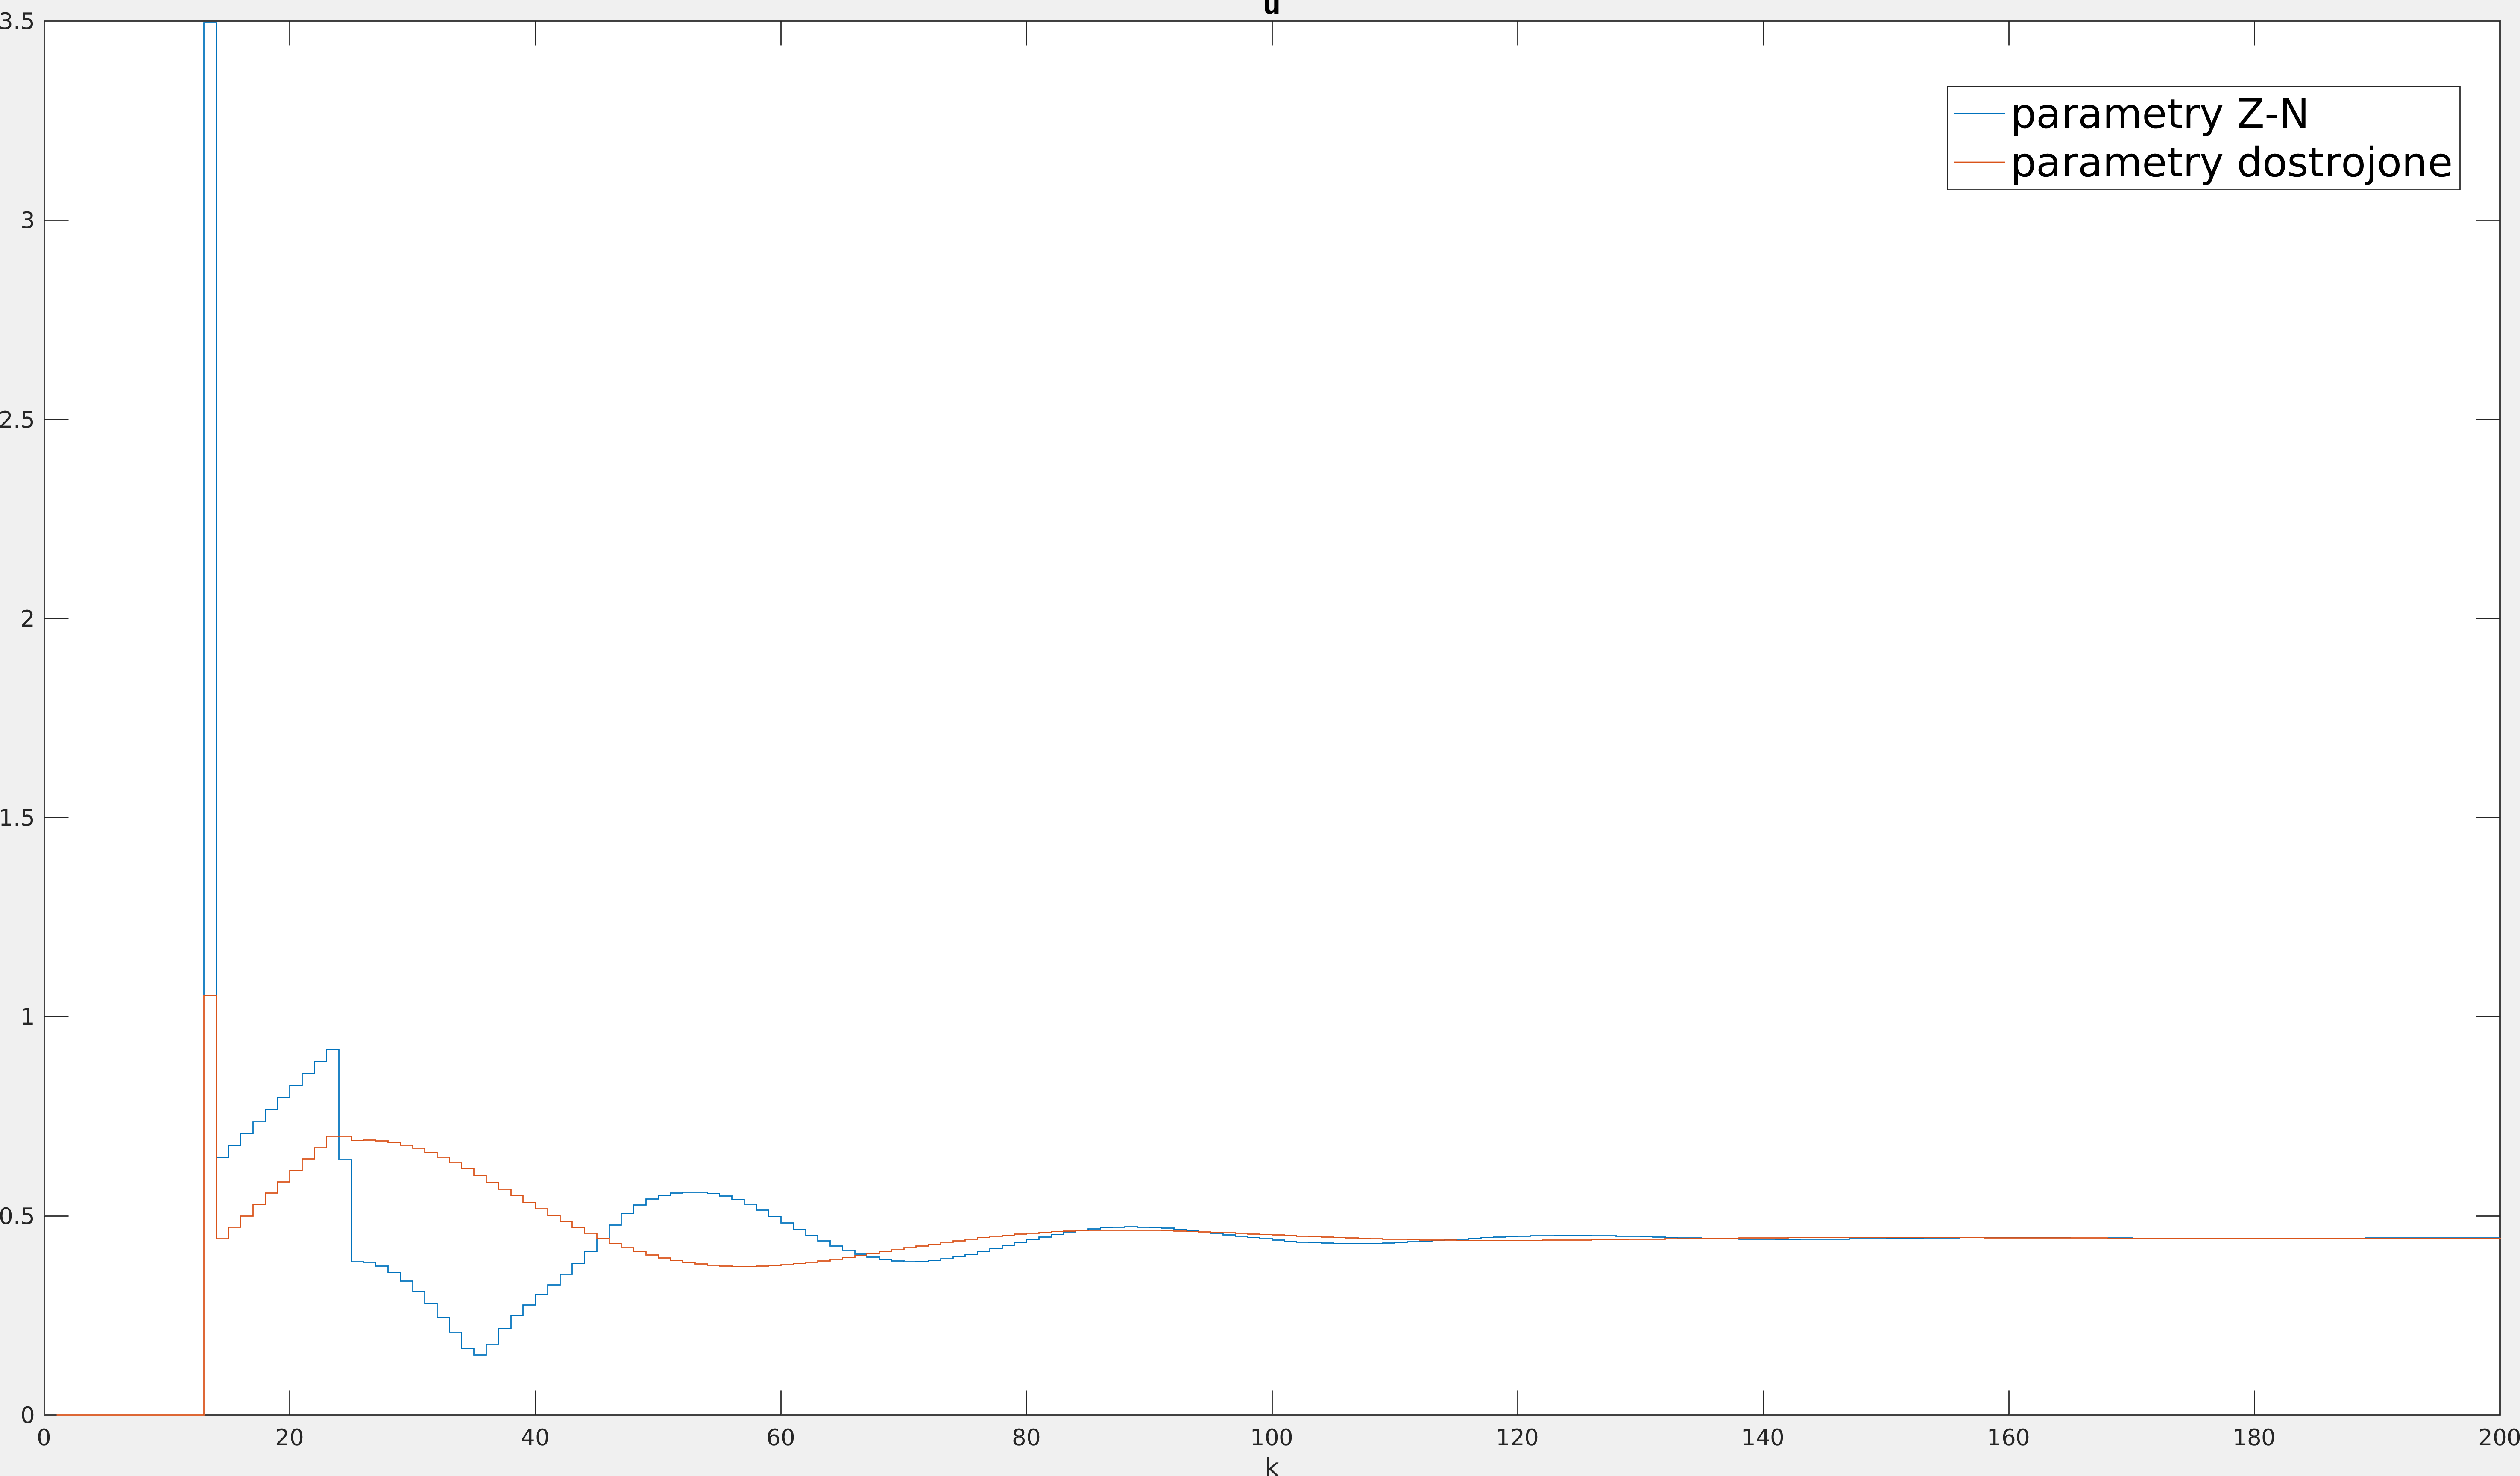
\includegraphics[width=\textwidth]{scripts/dyskretster.png}
	\caption{sygnał sterujący obiektu regulacji cyfrowej}
\end{figure}

Sygnał wyjściowy nie różni się zbytnio w przypadku początkowych nastaw i poprawionych, chociaż łagodniejsza odpowiedź i nieco krótszy czas regulacji przemawiają wciąż za wartościami dobranymi później. Dopiero wykres sygnału sterującego ukazuje zdecydowanie bardziej przyjazną trajektorię dla poprawionych współczynników, co ujawnia się trzykrotnie mniejszym skokiem sterowania na początku regulacji i łagodniejszym jego zmianom oraz szybszemu ustaleniu wartości.

\end{document}
